\chapter{Introduzione}
Il challenge di Machine Learning consiste nell’affrontare un problema di localizzazione basato su immagini, ovvero costruire un algoritmo che, data un’immagine acquisita in uno spazio noto, permetta di inferire la posizione dalla quale l’immagine è stata scattata.
\begin{figure}[H]
	\centering
	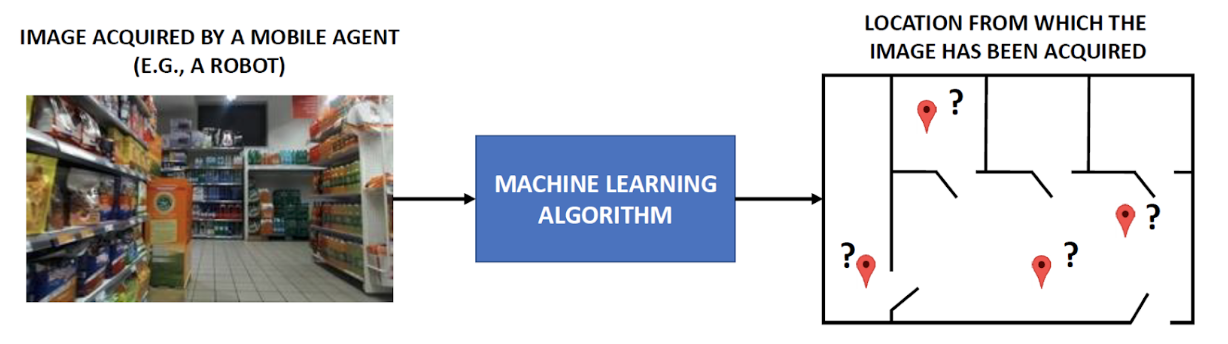
\includegraphics[scale=0.75]{image1.png}
\end{figure}
Esso può essere trattato come un problema di machine learning, e affrontato fondamentalmente in due modi:
\begin{itemize}
	\item[•]\bf Localizzazione basata su classificazione
	\item[•]\bf Localizzazione basata su regressione
\end{itemize}	
\begin{figure}[H]
	\centering
	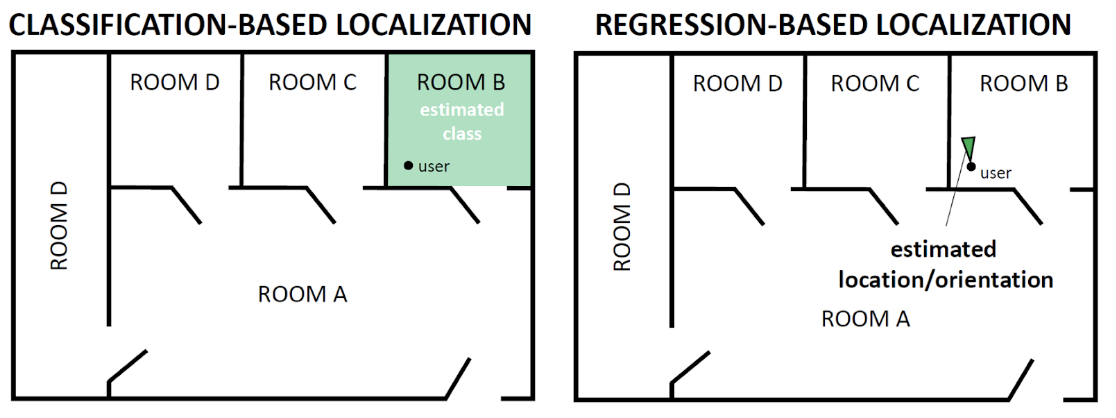
\includegraphics[scale=0.75]{image2.png}
\end{figure}
La sorgente dei dati in esame è una camera incorporata in un robot che effettua un determinato cammino in un supermercato. Il robot acquisisce un video che successivamente viene suddiviso nei suoi frames. Essi faranno parte del dataset.
\\
Il {\bf problema di classificazione} consiste nella localizzazione del robot in uno dei 16 reparti del supermercato.
\\
Il {\bf problema di regressione}, invece, consiste nel prevedere la posizione del robot nei momenti dell’acquisizione del video.
\newline
Il dataset quindi è formato dalle immagini e da un insieme di relative etichette che rappresentano rispettivamente:
\begin{itemize}
	\item[•] Posizione rispetto all’asse X
	\item[•] Posizione rispetto all’asse Y
	\item[•] Orientamente etichettato da U e V
	\item[•] Classe di appartenenza
\end{itemize}	
Per risolvere i problemi di classificazione e regressione abbiamo implementato e confrontato i seguenti algoritmi: {\bf MLP}, {\bf MLP Deep}, {\bf VGG16 pre-addestrata} con opportuno fine tuning. \\
Per l’esecuzione dei test è stata utilizzata la seguente configurazione hardware/software:
\begin{itemize}
	\item[-] {\bf O.S}: Ubuntu 18.04
	\item[-] {\bf CUDA}: v9.1.85
	\item[-] {\bf PyTorch}: v0.4
	\item[-] {\bf CPU}: Intel core i7 di 2° generazione
	\item[-] {\bf RAM}: 8 GB ddr3
	\item[-] {\bf GPU}: Nvidia geForce GTX 1080ti
\end{itemize}	
